\hyphenation{Life-long}
\section{The Neuroscience and Human-Performance Perspective on
Lifelong Learning} \shorttitle{Neuroscience and Human Performance
}

  Our research focuses on identifying mechanisms underlying cortical plasticity and the structure-function relationships between cognitive, sensory, and motor performance and learning. The human brain remains plastic even at high age. However, plastic capacity declines with age. In this context the ability to facilitate plasticity is of high significance for the elder learner.
  
 In this context, research of our group is divided into three main topics:

 Our first interest is to investigate the plastic-adaptive capacity of the brain to understand basic mechanisms of plasticity and learning as well as the effects of age. Based on these experiments possible interventions might be developed to improve learning and to interfere with age-related decline. Fields of research are vibrotactile perceptual learning, force control and force modulation, motor-cognitive dual-task performance, intermanual transfer of learned motor programs, and the sensory-motor coupling during learning.
	
 Second, physical fitness is assumed to preserve cognitive functioning and psychological well-being in older adults. However, the mechanisms, the dose-response-relationship and also effects of different types of exercise are not well understood. Following an interdisciplinary view on human performance that comprises motor, neurophysiological, and psychological expertise and methods, the second area of research deals with the role of aerobic and acrobatic exercise on cognitive performance and well-being across the lifespan.
	
 Third, the plastic-adaptive capacities of the adult and aging brain are of particular importance for the aging work force. As part of joint JCLL efforts, combining our expertise in the above mentioned fields of research, we developed a research proposal to establish measures of older workers' adaptivity in the sensory, motor and cognitive domains and to relate their adaptive capabilities to the demands of the work place. From the results we will be able to identify mismatches between demands of the work place and individual preconditions. We assume that these mismatches might be used as predictors of low productivity or health problems of the employees.

\subsection{Plastic-Adaptive Capacity of the Brain: Mechanisms, Effects of Age, Possible Interventions}


\index{Godde, Ben}

\paragraph{Research Team}
Ben Godde (Professor), Claudia Voelcker-Rehage (Postdoctoral Fellow), Mikhail Babanin (Doctoral Fellow), Alexander Knop (Diploma Student, University of Bremen).

First, within the sensory domain we are interested in the plastic-adaptive competencies related to tactile processing of younger and older adults. Using functional MRI and psychophysics we investigate the cortical topography of tactile perception and the cortical mechanisms of perceptual learning.
	
	Second, within the motor domain, we are mainly interested in upper extremity force control. Control of the fine finger forces is an elementary component of movement production of many daily activities (e.g. dressing, eating, opening containers) and its assessment provides insight into movement control and coordination. A decline in force control is common in older adults. We examine age-related differences in force control, practice effect on force modulation, and age-related differences in dual-task performance. Besides force control we are interested in the intermanual transfer of learned motor programs.
	
	In a third line of research we are going to focus on the interaction between motor and sensory performance. Particularly, we are interested in the following questions: (1) Does high frequency tactile stimulation help to diminish age-related performance decrements in force control? 
	
\newpage
(2) Does high frequency tactile stimulation facilitate sensory and/or motor learning? These questions are the first steps in developing appropriate interventions to improve manual dexterity in older adults.

\null
\textbf{Research Highlights 2006}


\textit{Effects of high frequency tactile stimulation on sensory and motor performance in younger and older adults}

	It is assumed that an important mechanism responsible for precise force control is tactile sensitivity. However, also contradictory results exist and the neural control mechanisms responsible for precise manipulation of grasping forces are largely unknown. We examined the link between motor and tactile domains by applying an intervention paradigm of high frequency ($\sim$20Hz) tactile stimulation (tHFS). This protocol is assumed to induce long-term potentiation (LTP) like effects in the neocortex and has recently been shown to profoundly improve tactile acuity. 

	Younger (18-28 years of age) and older (65-75 years of age) right handed participants were randomly assigned to an experimental and a control group. Before and after 30 minutes of tHFS on the index finger and thumb of the left hand, participants performed different tactile (spatial and temporal discrimination) and motor tasks (unimanual isometric precision grip task using a Mini Model force transducer and Purdue Pegboard test) with their stimulated fingers.
	
	Results indicated that tHFS significantly improved tactile frequency discrimination of the left index finger, whereas motor performance as assessed with the pegboard task was impaired (see Figure \ref{fig:profBenGodde}). These effects were found for both age groups with similar effect sizes even though absolute levels of performance in all tasks were lower for older as compared to younger adults. For the precision grip task younger subjects of both the experimental and control group similarly improved from the pre to the post test. Contrary, only older subjects which received the tHFS intervention could profit from the test repetition whereas the performance of the older control group remained stable. 
	
	Our results suggest that reorganization of the somatosensory cortex presumably induced by the applied protocol of passive tactile stimulation not only promotes sensory performance but also significantly affects fine motor control of the respective fingers. Moreover, our study reveals the remaining plastic capacity of the older brain (Voelcker-Rehage, Knop, Babanin \& Godde, 2006). 

%\begin{figure}[ht]
%  \begin{center}
%    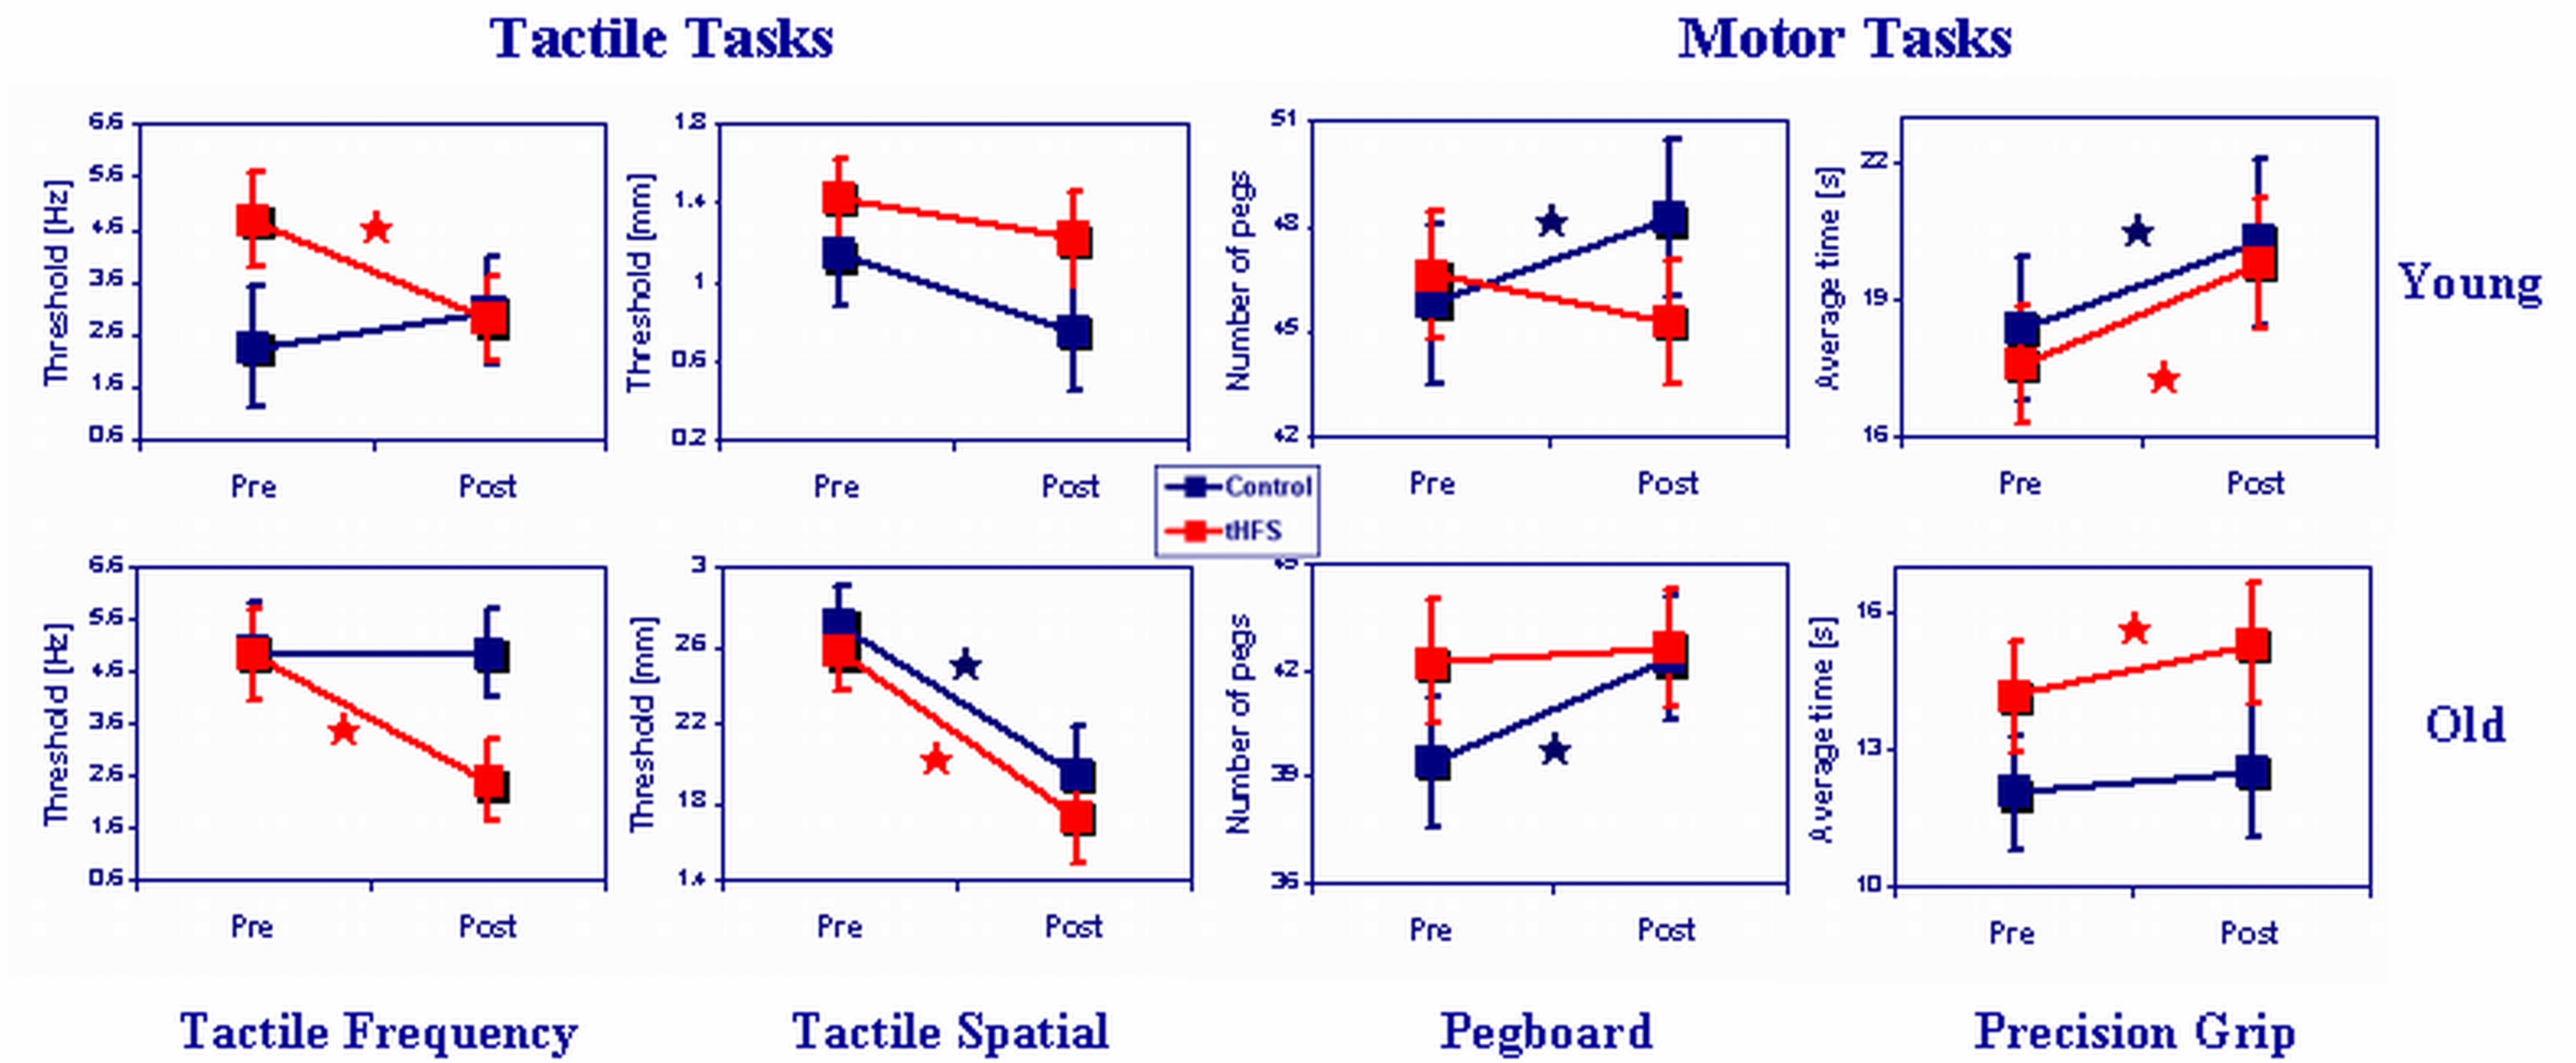
\includegraphics[width=7.5cm]{profBenGodde-fig1.jpg}
%    \caption{Differential effects of tHFS on tactile (left 2 columns) and motor (right 2 columns) performance in young %(top) and old (bottom) subjects. Experimental group shown in red, control group in blue.}\label{fig:profBenGodde}
%   \end{center}
%\end{figure}

\begin{figure}[htb]
  \begin{center}
    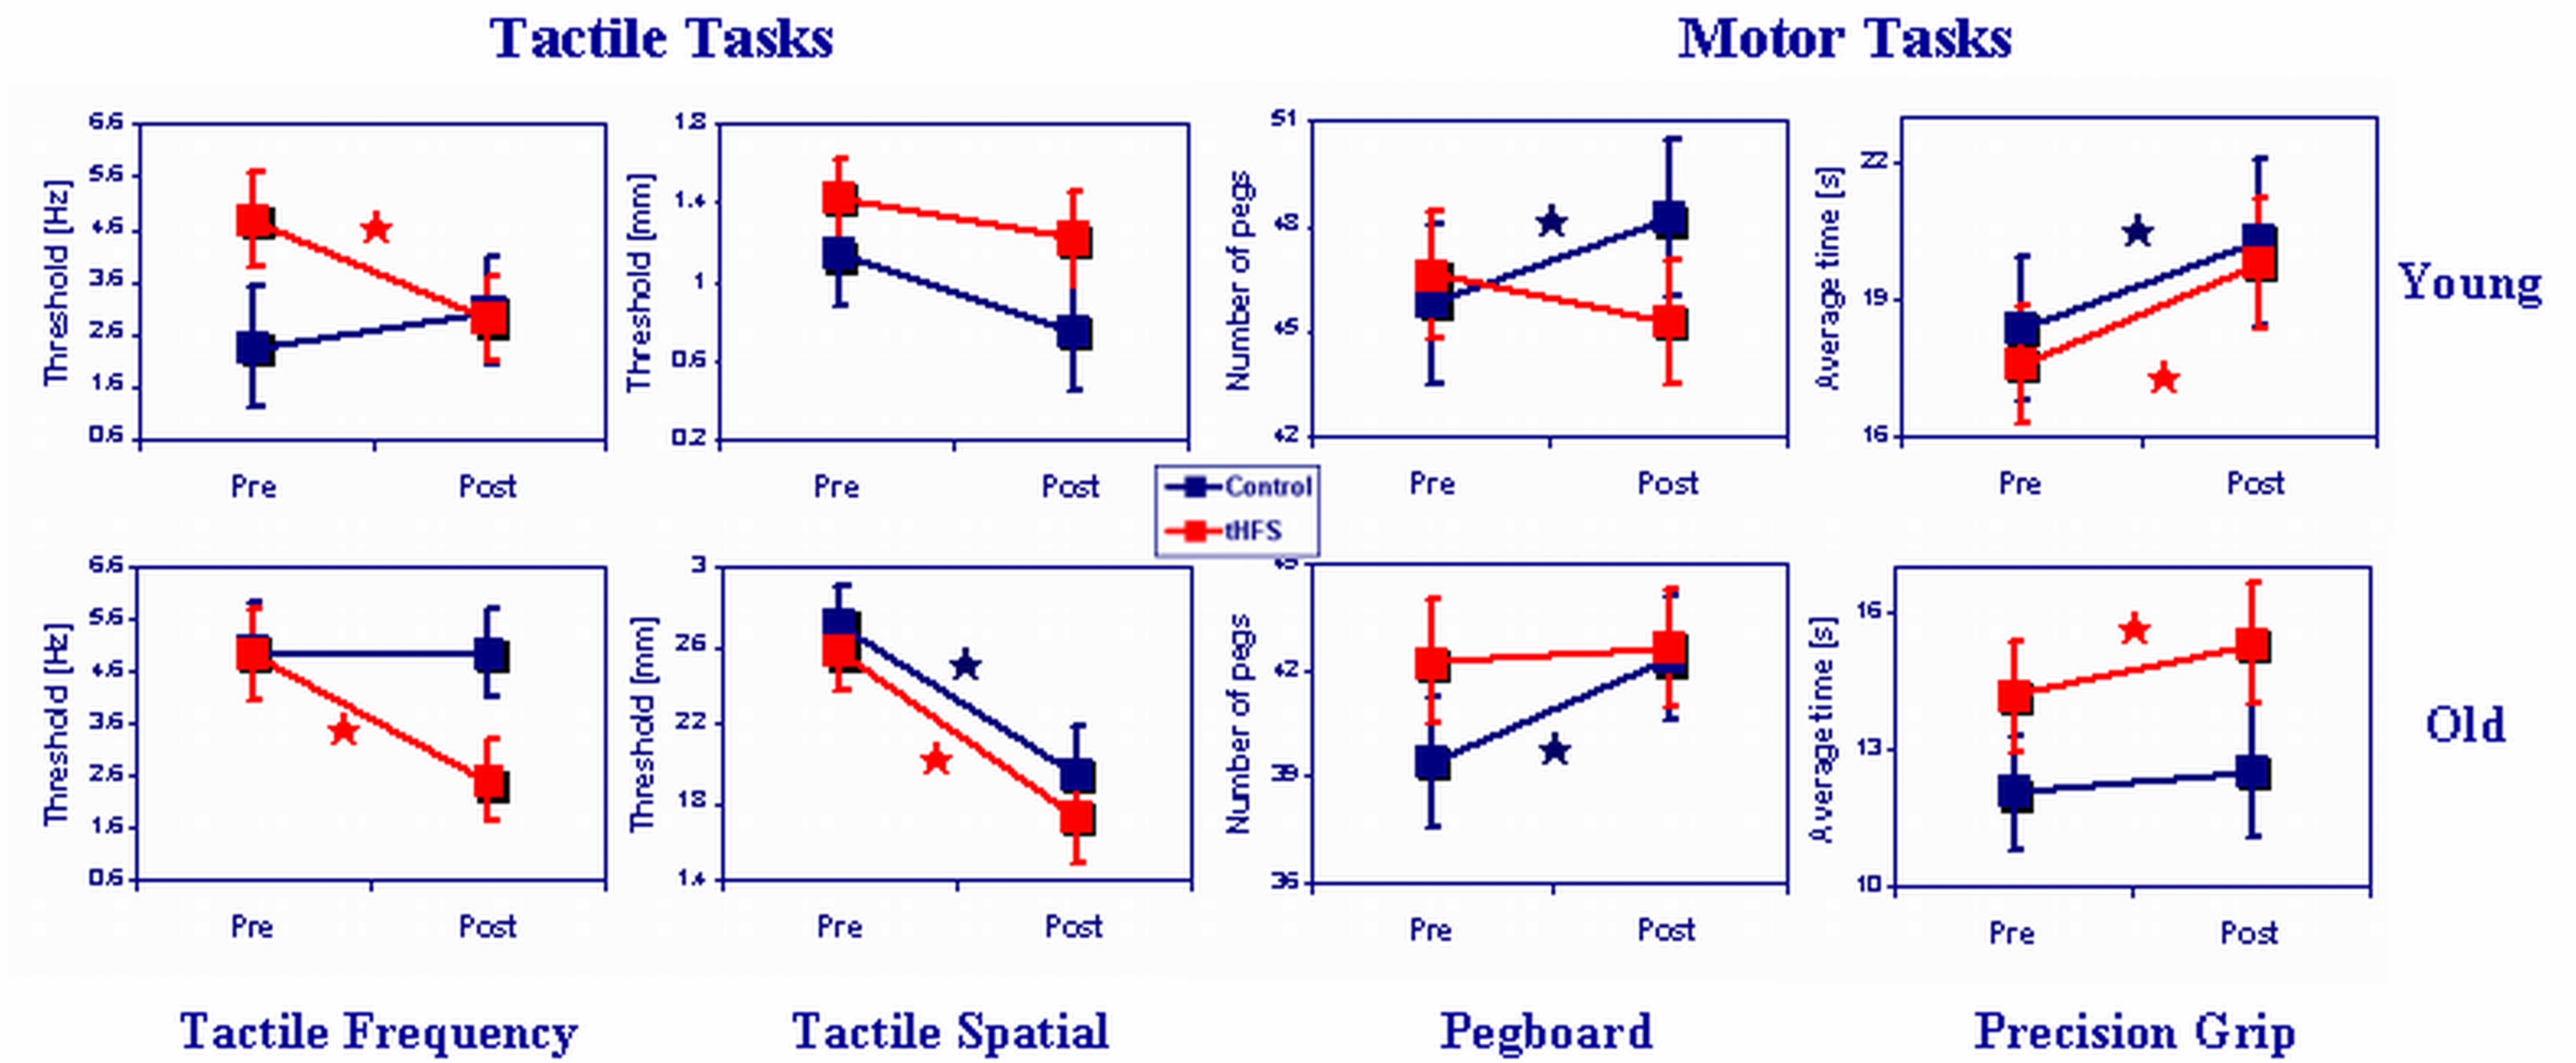
\includegraphics[width=0.5\textwidth]{profBenGodde-fig1}
    \caption{Differential effects of tHFS on tactile (left 2 columns) and motor (right 2 columns) performance in young (top) and old (bottom) subjects. Experimental group shown in red, control group in blue.}
    \label{fig:profBenGodde}
  \end{center}
\end{figure}




\enlargethispage*{0.2cm}
\paragraph{Collaborations}
\begin{itemize}
\item University Hospital T\"{u}bingen \\ MEG-Center \\ PD Dr. Christoph Braun 
\item University of T\"{u}bingen \\ Medical Psychology and Behavioral Neurobiology \\ Dipl-Psych. Ahmed A. Karim
\item International School for Advanced Studies \\ Trieste, Italy \\ Cognitive Neuroscience Sector \\ Prof. Mathew E. Diamond, PhD
\item Lerner Research Institute, USA \\ Department of Biomedical Engineering \\ Cleveland Clinic Foundation \\ Jay L. Alberts, PhD
\item IUB, SES \\ Prof. Dr. Claus Hilgetag
\item University of Bremen \\ Interdisciplinary Center for Cognitive Sciences \\ Prof. Dr. Manfred Herrmann; Prof. Dr. Manfred Fahle
\end{itemize}

\begin{bibunit}[apalike]
\nocite{*}
\putbib[profBenGodde1]
\end{bibunit}

\paragraph{Grants}
\begin{itemize}
\item DFG (submitted; PI: C. Voelcker-Rehage in cooperation with Jay L. Alberts, PhD, Cleveland Clinic Foundation, USA): Age-related changes in functional uni- and bimanual dexterity; grasping force modulation in older adults.

\item BMBF (PI: JCLL). B. Godde, C. Voelcker-Rehage: subproject ``Adaptive Competence'' within the joint research project ``Effects of Matches/Mismatches between Aspects of Human and Social Capital, Corporate Strategy and Work Organization on the Physical and Mental Well-Being of Employees''. 
 
\end{itemize}

\subsection{Effects of Cardiovascular and Motor Fitness on Cognitive Performance and Well-Being in Older Adults}


\index{Godde, Ben}

\paragraph{Research Team}
Claudia Voelcker-Rehage (Postdoctoral Fellow), Ben Godde (Professor), Ursula M. Staudinger (Professor), Mikhail Babanin (Doctoral Fellow), Kathrin Linke (Diploma Student), Tanja Truhart (Student, University Bremen), Silja Menken (Student, University Marburg), Pit Peltz (Student, University Bremen).

Following an interdisciplinary view on human performance that comprises motor, neurophysiological and psychological expertise and methods, our second area of research deals with the role of cardiovascular fitness and motor coordination training on cognitive performance and psychological well-being in older adults. More and more animal and human studies stress the importance of a physically active lifestyle for successful aging (i.e. retarded cognitive decline, improved physiological and psychological health etc.). However, the underlying mechanisms, the dose-response-relationship and also the effects of different types of exercise on cognitive performance are still not well understood.

\null
\textbf{Research Highlights 2006}

 Currently we are performing a one-year longitudinal study to investigate the effect of different types of physical activity on cognitive performance and well-being in older adults. 
\newpage 
This study started in October 2006 and results of baseline measurement are just under investigation. In preliminary studies we developed and evaluated training programs and test batteries for practicing and assessing gross and fine motor coordination in older adults. We also performed a pilot cross sectional study on the effects of different types of physical exercise (endurance training, strength training, mixed training) on cognition and well-being. 

\begin{figure}[h]
  \begin{center}
    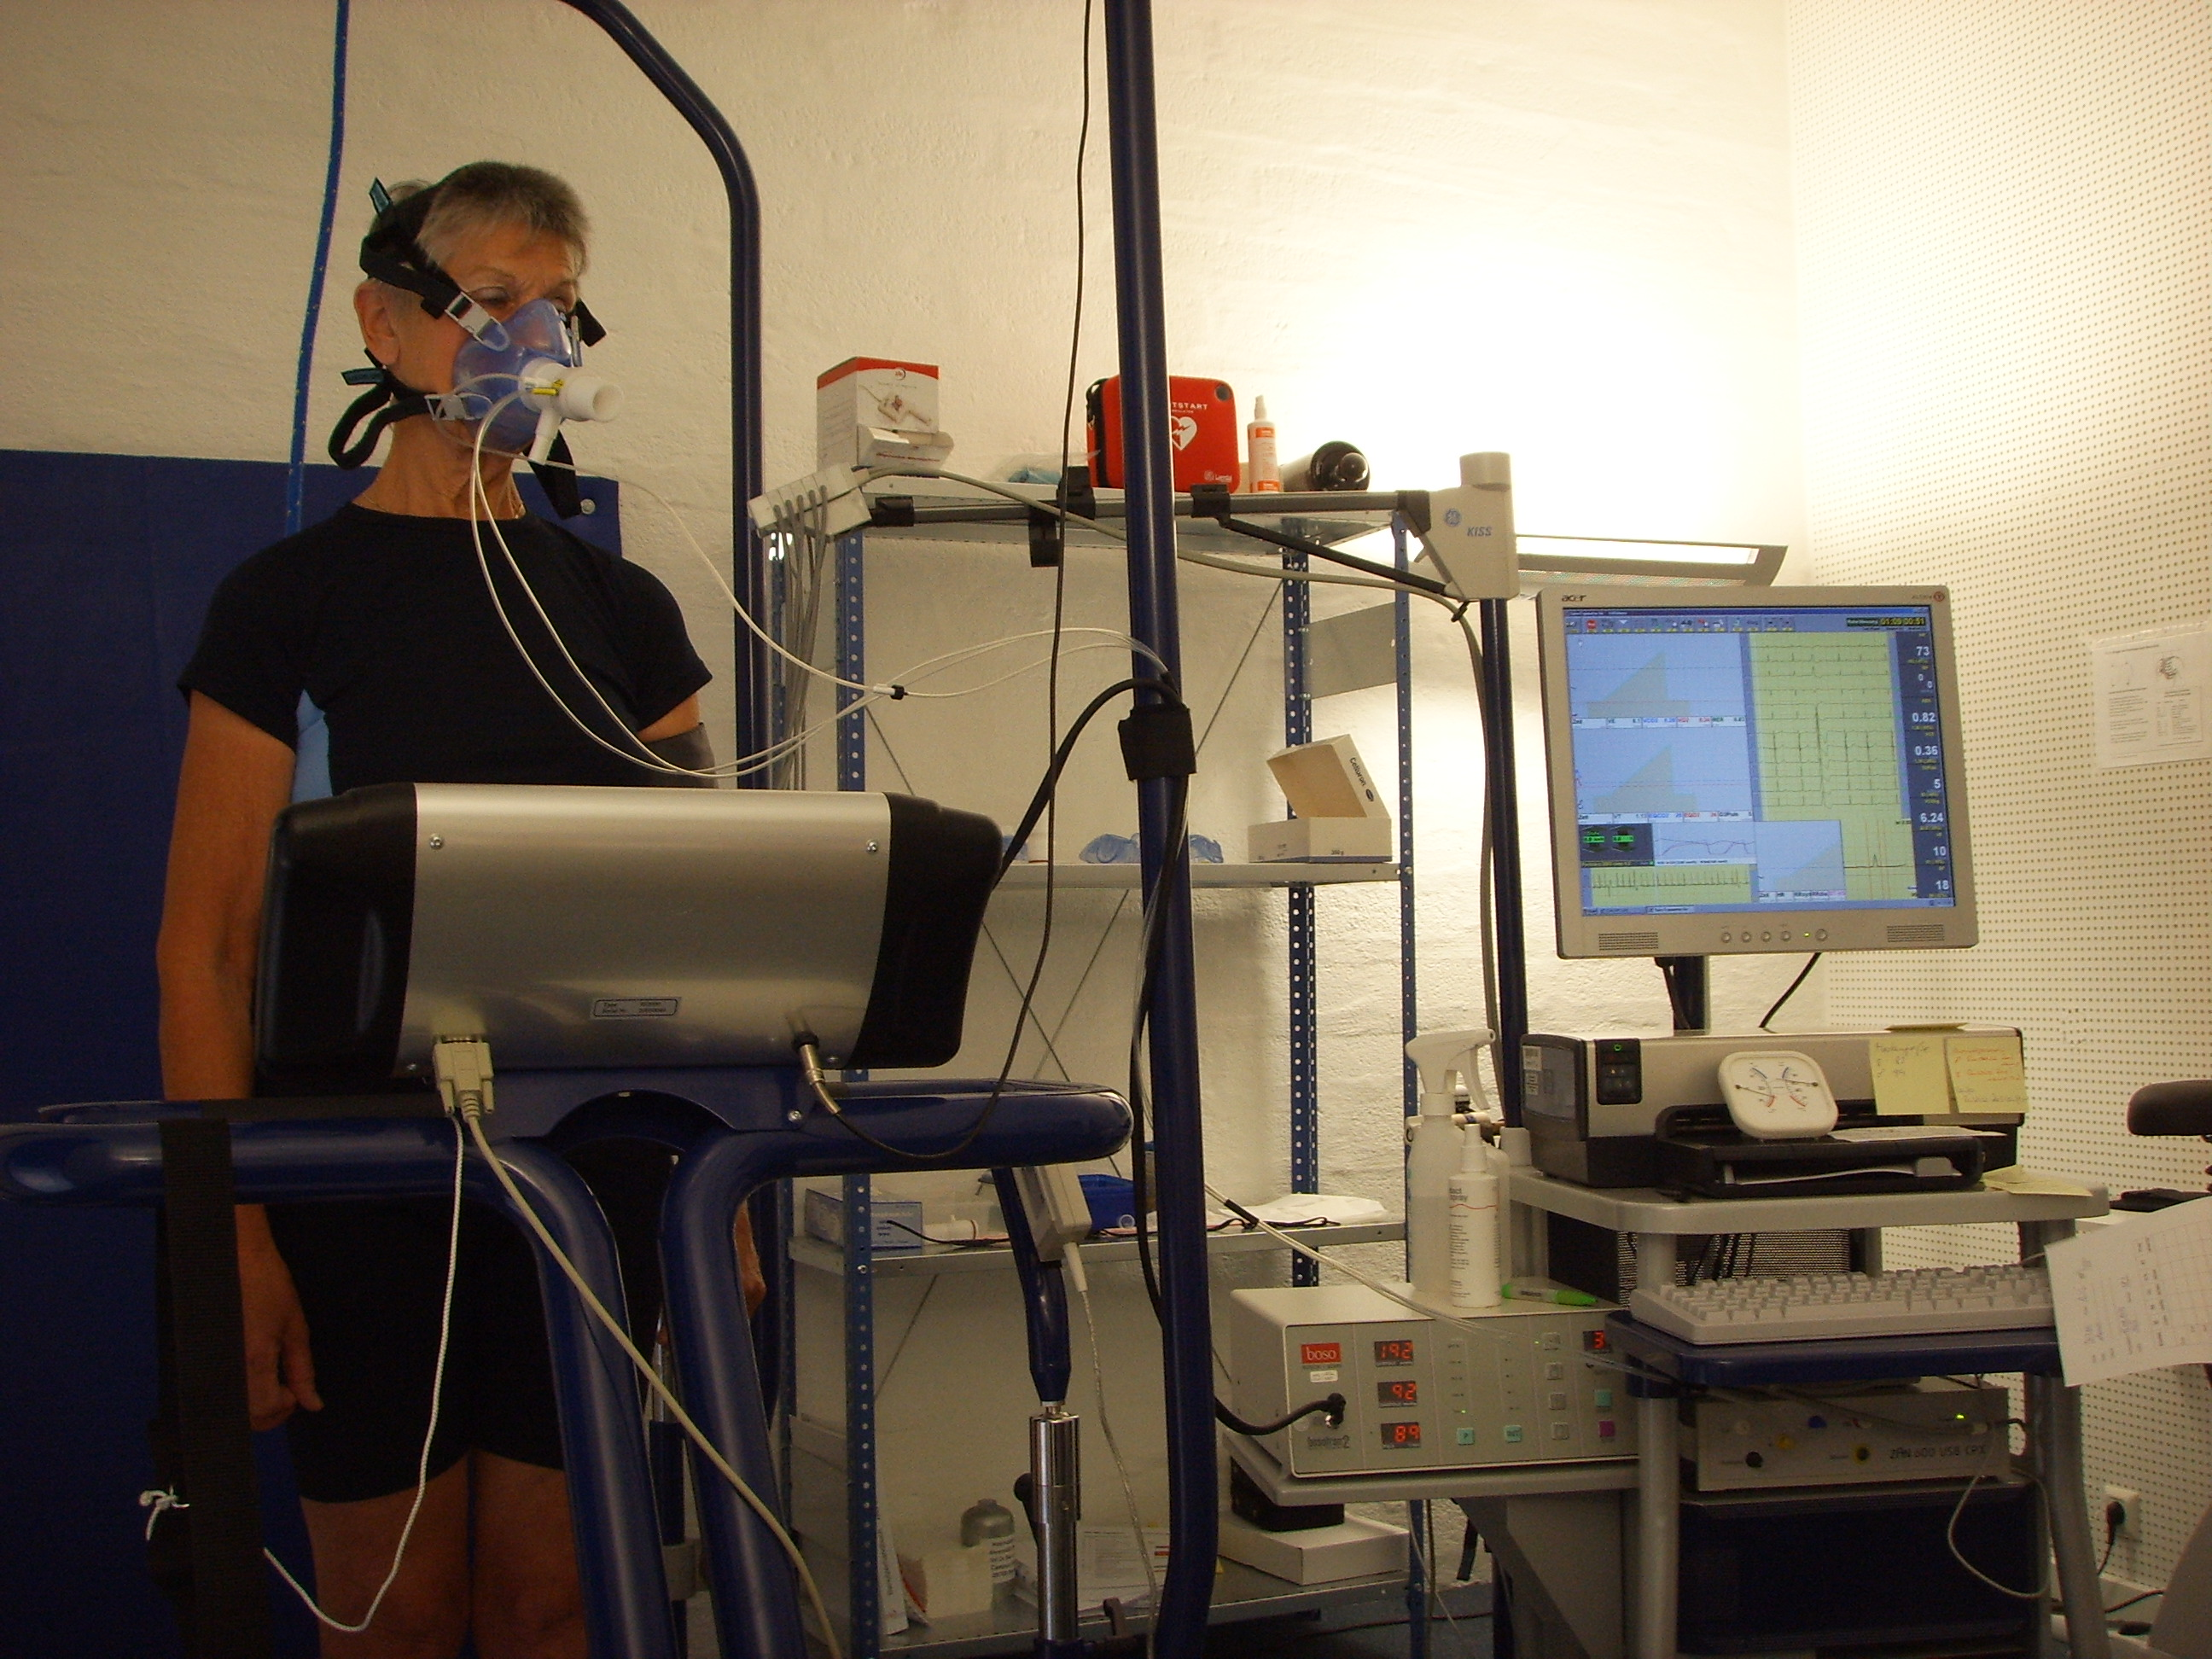
\includegraphics[width=7.5cm]{profBenGodde-fig2.jpg}
    \caption{Using a ZAN600 spiroergometric system (ZAN Messtechnik, Oberthulba, Germany) we measure the cardiovascular and respiratory fitness of participants to develop individual recommendations for their training programs.}\label{fig2:profBenGodde}
   \end{center}
\end{figure}

\textbf{Collaborations}
\begin{itemize}
\item University of Bielefeld \\ Department of Sports Science \\ Prof. Dr. Klaus Willimczik
\item University of Bremen \\ Movement Science and Training\\ Sports Science \\ Dr. Monika Fikus
\item University of Bremen \\ Interdisciplinary Center for Cognitive Sciences \\ Prof. Dr. Manfred Herrmann
\item IUB, JCLL \\ Prof. Dr. Ursula M. Staudinger
\end{itemize}

\begin{bibunit}[apalike]
\nocite{*}
\putbib[profBenGodde2]
\end{bibunit}

\paragraph{Grants}
\begin{itemize}
\item Robert Bosch Foundation \& German Health Insurance Company (PI: C. Voelcker-Rehage in cooperation with B. Godde and U.M. Staudinger, JCLL, IUB): Facilitating Motor and Cognitive Performance in Old Age.
\item DFG travel grant for C. Voelcker-Rehage, Society for Neuroscience Annual Meeting, October 14-17, 2006, Atlanta, GA, USA.
\item DFG travel grant for C. Voelcker-Rehage, Annual meeting of the North American Society for Psychology of Sport and Physical Activity, June 9-11, 2006, St. Petersburg Beach, FL, USA.
\end{itemize}





\subsection{Awards, Fellowships}

\begin{itemize}
\item Junior Fellow of the Leopoldina-Acatech Working group ``Chancen und Probleme einer alternden Gesellschaft: Die Welt der Arbeit und des lebenslangen Lernens'' (Claudia Voelcker-Rehage).
\end{itemize}
 
\subsection{Other Professional Activities}

\textit{Ad-hoc Reviews}

\begin{itemize}
\item Godde, B.: \\Journal of Cognitive Neuroscience; Cognition; Quarterly Journal of Experimental Psychology, Journal of Neuroscience, Neuroscience and Biobehavioral Reviews; Experimental Brain Research; Journal of Neuroscience Methods; ACM Transactions on Applied Perception; Behavioural Brain Research.
\item Voelcker-Rehage, C.: \\European Review of Aging and Physical Activity.
\end{itemize}

